Descripción de la etapa de adquisición, sus partes, su relación con la etapa anterior, contenidos del capitulo.

\section{Arquitectura propuesta}
\label{sec:arq}

En el capítulo anterior, se compararon tres sistemas diferentes para la implementación de adquisición de datos para física de partículas. En ellos destacan aspectos comunes de implementación: etapas de detección de eventos, memorias para almacenamiento temporal, procesamiento de los datos y la utilización de FPGA como herramienta principal para la implementación del hardware.

¿Cuáles son las etapas esenciales que un DAQ debe poseer? En esencia se requiere de una primera etapa de interfaz de lectura directamente de los detectores (\textit{Readout}), las cuales suelen poseer amplificadores, modeladores de pulsos, memorias y digitalizadores. Una segunda etapa suele consistir en el preprocesamiento de las señales, extrayendo la información básica y formando estructuras de datos pertinentes. Finalmente, está la etapa de procesamiento fuera del detector, donde se realiza el análisis e interpretación de los datos.

En este proyecto de titulación, la primera etapa la lleva a cabo la tarjeta acondicionadora ASD (Amplifier Shaper Discriminator), diseñada para detectores del proyecto ATLAS. Las etapas restantes serán diseñadas pensando en la aplicación específica de este proyecto.



\subsection{Esquema General}
	Como se indica en la figura \ref{img:diagrama}, se requieren al menos tres etapas esenciales: discriminar, procesar y analizar. Discriminar se refiere a distinguir entre aquellos eventos que corresponden un muón de aquellos que no, descartando estos últimos. Procesar implica utilizar los pulsos escogidos, formar una estructura que los relacione como un solo evento y posiblemente incluir información de ellos, como una marca temporal y la duración de los pulsos captados en dicho evento. 
	
	\begin{figure}[h]
		\centering
		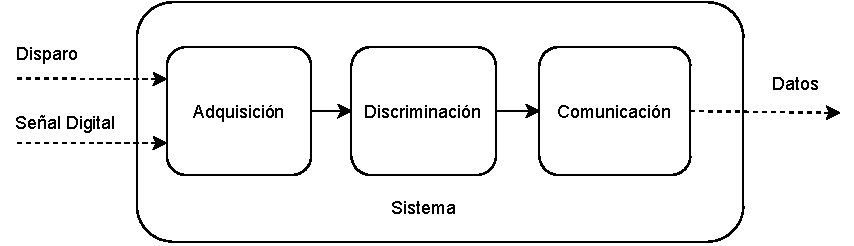
\includegraphics[scale=0.9]{basico.pdf}
		\caption{El disparo corresponde a la señal digital que indica si la partícula detectada es un muon, mientras que la señal digital corresponde al pulso captado por el detector, luego de haber pasado por la interfaz de lectura.}
		\label{img:diagrama}
	\end{figure}

	La etapa de análisis implica mayor complejidad y puede extenderse para abarcar distintos niveles. El análisis más básico implica leer un evento e inferir la región del detector que fue excitada por el paso del muon. Niveles siguientes implicarían estimar la energía del muon, incluir mayor precisión espacial, correlacionar con eventos anteriores o incluso trazar la trayectoria  del paso de la partícula al superponer los datos de eventos originados en otros detectores.

\newpage
\subsection{Requisitos}
	
	\begin{itemize}
		\item Se debe contar con al menos 32 pares de entradas bajo el estándar LVDS, con el fin de conectar al menos 2 tarjetas ASD (Amplificator Shaper Discriminator) utilizadas cada una como la interfaz de detectores de 16 canales.
		\item Es importante contar con un reloj presente o sintetizable de una frecuencia mayor a 100[MHz], lo más cercano a 1[GHz] posible, con el fin de captar la duración de los pulsos y el momento de aparición de un evento con la mayor precisión disponible.
		\item Se debe considerar que la señal de disparo que entrará al sistema estará desfasada cerca de 100[ns] respecto al paso real de los muones por el detector, siendo necesaria la implementación de delays para las señales capturadas o un sistema capaz de distinguir la ocurrencia de eventos y disparos en el tiempo.
		\item  Se debe tener la capacidad de mantener señales sincronizadas, guardar información en memorias temporales y llevar cuenta del transcurso del tiempo entre eventos.
		\item Es requisito que la implementación de la alternativa permita escalamiento para agregar nuevos detectores adyacentes con el fin de aumentar el área de prueba, así como también sincronizarse con detectores paralelos para trazar trayectorias de las partículas captadas.
	\end{itemize}
	
	En cuanto a los requisitos de tiempo y reloj de operación anteriormente indicados, estos se deben esencialmente a que la duración de un pulso digital proveniente de un detector podría estar entre 1[ns] y 40[ns]\cite{1999ATLASICs}. Este ancho de pulso tiene correlación con la amplitud del pulso análogo original y el error en su medición implicará menor precisión en la estimación de esta variable.
	
	Respecto a la tasa de aparición de pulsos consecutivos, es poco probable que ocurran eventos simultáneos o cercanos. Se espera que la tasa de muones por centímetro cuadrado sea de un muón por minuto, lo que en los $15[cm^2]$ representados por una señal de detector implicaría cerca de 15 muones por minuto o $2,5*10^{10}$ muones cada 100 [ns], lo que se traduce a una muy baja probabilidad de eventos simultáneos o incluso cercanos. De hecho, la tasa de detección de muones puede disminuir estando bajo tierra y se planea que la toma de una muongrafía conlleve un tiempo prolongado de exposición a rayos cósmicos. Esto conduce a la conclusión de que ignorar posibles eventos simultáneos o adyacentes no tendrá implicancias significativas en los resultados de la muongrafía final.

\newpage
\subsection{Propuesta}
	La alternativa más utilizada en el rubro es la FPGA. Esta ha sido la herramienta que se ha visto con mayor frecuencia en proyectos relativos a física de partículas y adquisición de datos. 
	Las FPGA cuentan con una cantidad significativa de recursos y periféricos. Incluyen además hardware dedicado para comunicación, serialización y almacenamiento de datos. Incluso suelen incluir CPLDs en las placas que las albergan. Una desventaja conocida corresponde a que se basan en memorias volátiles, por lo que el hardware descrito se debe reconfigurar cada vez que se enciende, y los datos importantes deben ser almacenados en memorias externas.
	
	Para esta alternativa se propone el uso de la tarjeta de desarrollo Trenz TR0712 \cite{TrenzElectronic2019TR07012Wiki} montada en una placa TR0703 \cite{TrenzElectronic2019TR0703Wiki}. Esta tarjeta en su conjunto se basa en una FPGA Xilinx Artix 7 \cite{Xilinx20107DS180} de cerca de 16.000 celdas lógicas, incluyendo además chips de memoria RAM, reloj de 20[MHz] con hasta 600[MHz] sintetizables, comunicación Ethernet y por supuesto puertos LVDS suficientes para conectar al menos 2 detectores.
	
	Si bien esta tarjeta cuenta con puertos LVDS, será necesario confeccionar un adaptador para conectar las señales del detector hacia la placa Trenz.
	
	La frecuencia de reloj que puede alcanzar esta tarjeta es mucho mayor que cualquiera de las anteriores, siendo entonces la que permite tener mayor precisión en términos de tiempo, sobretodo para determinar la duración de los pulsos provenientes del detector.
	
	La idea en esta alternativa de solución es guardar los datos en memoria temporal hasta la llegada de una señal de disparo. Un módulo que maneja la memoria será el encargado de tomar los pulsos correspondientes al disparo recibido y liberar la memoria de aquellos datos ya leídos u obsoletos, entregando la información útil a una siguiente etapa. Los pulsos aceptados serán entonces relacionados como parte de un mismo eventos y se estimará la duración de estos, generando y guardando así un arreglo de datos con identificador de pulso y duración. La última etapa se encargará de efectuar una operación capaz de determinar la posición del evento a partir de las duraciones medidas y los pulsos detectados, comunicando así un arreglo básico y preprocesado que incluya posición y magnitud aproximada.
	
	\par Se espera que para lograr el escalamiento se incluya una señal para mantener la lectura de eventos sincronizada entre distintas FPGA. Además, se deberá incluir un modulo de comunicación para entregar la información captada a una etapa posterior con un análisis más detallado, encargado de reunir todos los eventos de diferentes FPGAs.
	
	\newpage
	\par Las figuras \ref{img:fpga1} \ref{img:fpga2} ilustran conexiones y bloques a implementar en esta alternativa de solución.
	
	\begin{figure}[H]
		\centering
		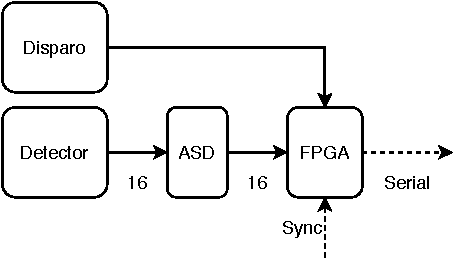
\includegraphics[scale=1]{fpga1.pdf}
		\caption{Diagrama de bloques utilizando una FPGA como alternativa de solución. Se indica una salida serial para transmitir los resultados del análisis básico a algún procesador o memoria de alguna etapa posterior. La señal de sincronización, inspirada en la alternativa \ref{sec:micro} tiene como objetivo sincronizar la recolección y procesamiento de eventos, para que estos sean consistentes entre detectores.}
		\label{img:fpga1}
	\end{figure}
	
	\begin{figure}[H]
		\centering
		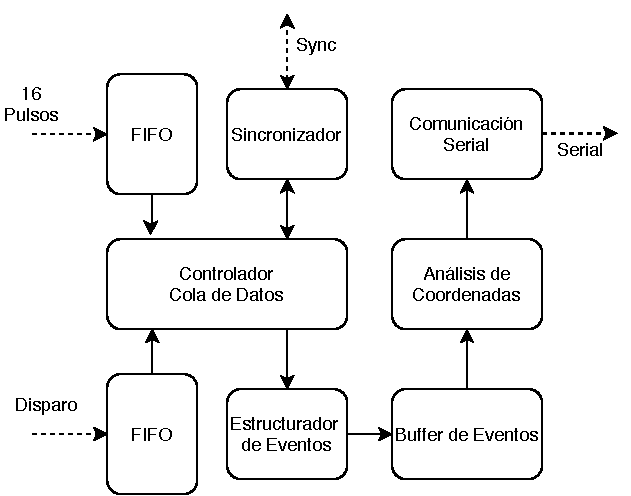
\includegraphics[scale=1]{fpga2.pdf}
		\caption{Representación de la lógica interna de la FPGA. Se agrega una cola de datos para las señales de disparo y una memoria de almacenamiento temporal para los eventos ya estructurados. Ambas implementaciones permiten tener mejor control del flujo de datos, evitando perdidas y asegurando sincronía a pesar de que la lectura de la información sea eventualmente más lenta que la captura de pulsos. Los bloques controlador, estructurador y análisis cumplen las mismas funciones mencionadas en alternativas anteriores: aceptar o descartar pulsos, cuantificar anchos de pulso a  los canales asociados y determinar coordenada del cruce de un muón respectivamente.}
		\label{img:fpga2}
	\end{figure}
	
	\newpage
	\subsubsection*{Atributos}
	\begin{itemize}
		\item \textbf{Simplicidad:}  \textit{6 - Media}. Gran cantidad del sistema concentrado en una sola placa, pero aumenta la dificultad en la descripción de hardware.
		\item \textbf{Desempeño:}  \textit{9 - Alto}. Gran cantidad de recursos lógicos, de almacenamiento y con alta  frecuencia de operación (600MHz máximo).
		\item \textbf{Disponibilidad: } \textit{9 - Alta}. Se cuenta con una en el laboratorio, pero se necesitarán un par de elementos para interconectarla con la placa ASD.
		\item \textbf{Economía: }\textit{6 - Media}. Una tarjeta de desarrollo de este estilo tiene un costo de aproximadamente US\$400.
		\item \textbf{Flexibilidad:} \textit{10 - Alta}. Alta flexibilidad en análisis, procesamiento y adquisición.
		\item \textbf{Documentación:} \textit{8 - Alta} Existe gran cantidad de documentación del fabricante. Además, cuenta con una FPGA Artix 7 ampliamente conocida.
	\end{itemize}
	
	
	\subsubsection*{Ventajas}
	\begin{itemize}
		\item Gran cantidad del sistema concentrado en una sola placa.
		\item Escalable
		\item Cuenta con puertos LVDS
		\item Alta densidad de recursos lógicos
		\item Dispone de memoria suficiente para almacenar eventos
		\item Posee una alta frecuencia de reloj sintetizable, mejorando precisión temporal.
		\item Placa con muy buena documentación.
	\end{itemize}
	
	
	\subsubsection*{Desventajas}
	\begin{itemize}
		\item Se requiere confeccionar un adaptador para conectar el detector con la tarjeta de desarrollo.
		\item Se complica el diseño y la implementación del hardware.
	\end{itemize}
	

Esta alternativa fue seleccionada por sobre las demás debido a su destacado desempeño, ya que cuenta con mayor frecuencia de reloj disponible, gran cantidad de recursos y suficientes puertos LVDS. Este último requerimiento es necesario para recibir los pulsos digitales capturados por la interfaz ASD\cite{1999ATLASICs} provenientes del detector, los cuales se emiten bajo el estándar LVDS para transmisión de señales diferenciales.

Destaca también esta alternativa al ser una plataforma flexible, en sentido de brindar las posibilidades de adaptar el diseño propuesto sin tener que adquirir nuevo equipamiento. Esta versatilidad es intrínseca de las FPGAs, las cuales se caracterizan por permitir un gran control en el diseño del hardware a bajo nivel.

Por último, destaca por la información disponible que existe para operarla. Esta FPGA es ampliamente conocida y además está incluida en un módulo Trenz TR0712\cite{TrenzElectronic2019TR07012Wiki} montada en una tarjeta Trenz TR0703\cite{TrenzElectronic2019TR0703Wiki} que da acceso a la mayoría de sus puertos y recursos. Ambos elementos cuentan con buena documentación, incluyendo diagramas de conexiones detallados, los cuales facilitarán la descripción del hardware y la interconexión con el detector de muones.

\begin{figure}[H]
	\centering
	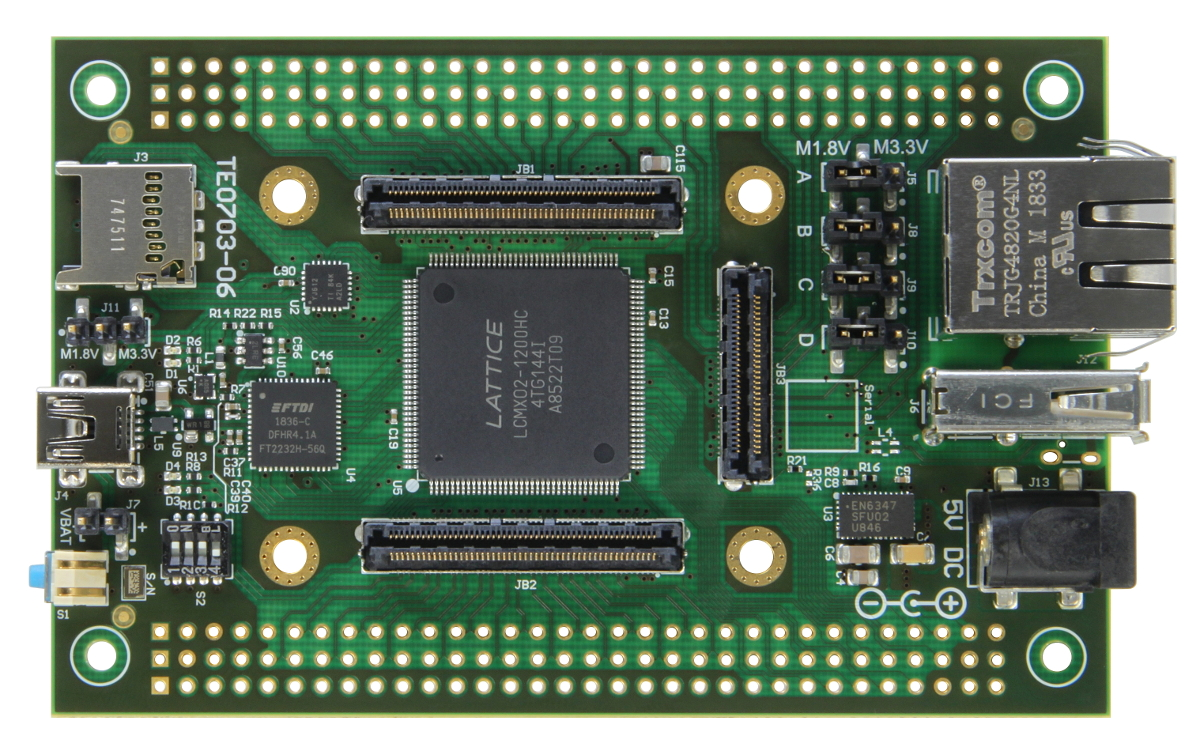
\includegraphics[scale=0.23]{TE0703-06_1.jpg}
	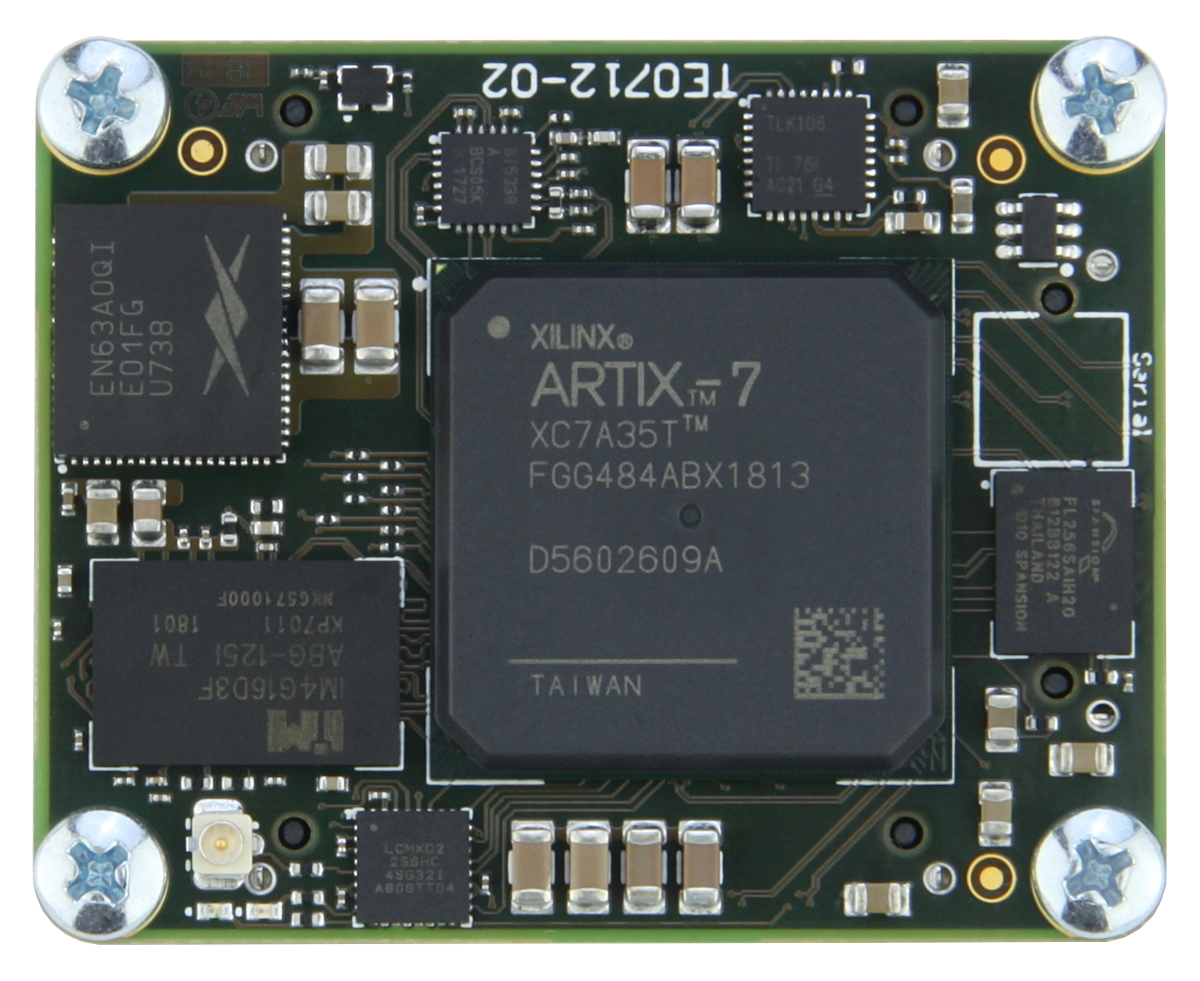
\includegraphics[scale=0.13]{TE0712-02-35-2I_1.jpg}
	\caption{Placa de desarrollo y módulo FPGA a utilizar. A la izquierda se ilustra la placa de desarrollo Trenz TR0703\cite{TrenzElectronic2019TR0703Wiki} y a su derecha se ilustra el módulo que va montado en ella: Trenz TR0712\cite{TrenzElectronic2019TR07012Wiki} que contiene una FPGA Artix 7\cite{Xilinx20107DS180}.}
	\label{fig:trenz}
\end{figure}


Para esta alternativa de solución se consideran 32 canales de entrada LVDS ya que en el futuro será necesario conectar al menos 2 detectores de 16 canales en una misma FPGA. Para este proyecto en particular se probará el sistema con un solo detector de muones, por lo que la prueba e integración de un segundo detector queda pendiente y no se implementará en esta etapa. La figura \ref{fig:ministgc} ilustra los canales que posee un solo detector de muones de $15cm^2$.

\begin{figure}[H]
	\centering
	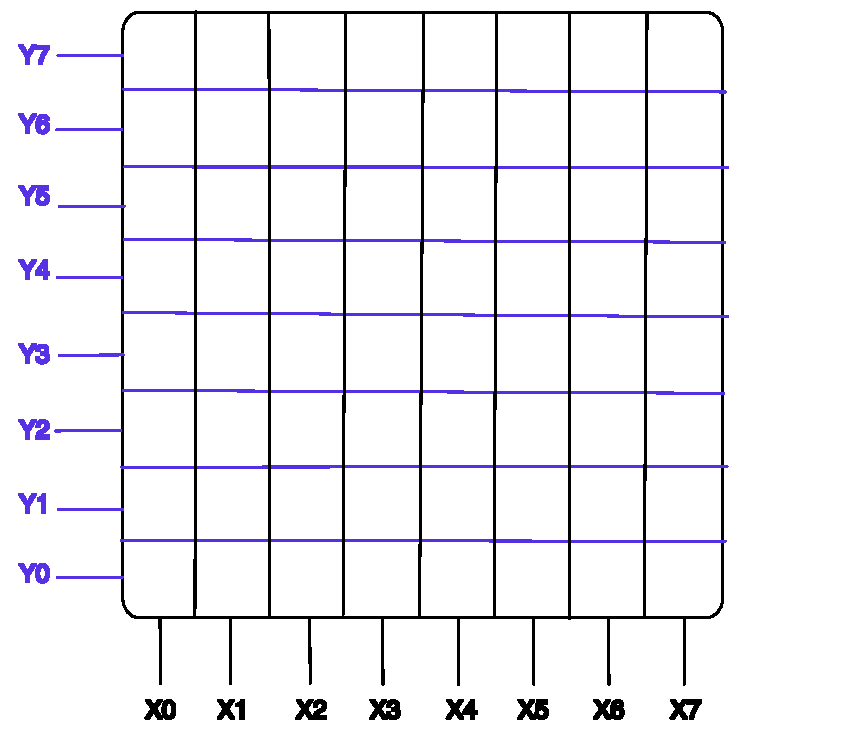
\includegraphics[scale=0.5]{cuadrantes-ministgc.pdf}
	\caption{Esquema de los canales provenientes de un detector Mini sTGC. Posee 8 tiras adyacentes de 15cm de largo por 1cm de ancho para cada eje coordenado. Cada tira emitirá un pulso analógico si una partícula cargada pasa través de ella. Se emitirán también pulsos de menor amplitud para el caso en que la partícula pase por una tira adyacente del mismo eje coordenado dentro de un radio específico. Este detector se posiciona perpendicularmente respecto a la fuente de radiación y en paralelo a (por debajo o por sobre) el sistema de disparo que indicará si la partícula captada corresponde o no a un muón. }
	\label{fig:ministgc}
\end{figure}

Las señales generadas por un detector son adaptadas por una tarjeta de interfaz ASD\cite{1999ATLASICs}, ilustrada en la figura \ref{fig:asd}. Esta tarjeta es capaz de capturar 16 señales simultaneas, por lo que es hardware suficiente para captar las señales de ambos ejes de un solo detector de muones.

\begin{figure}[H]
	\centering
	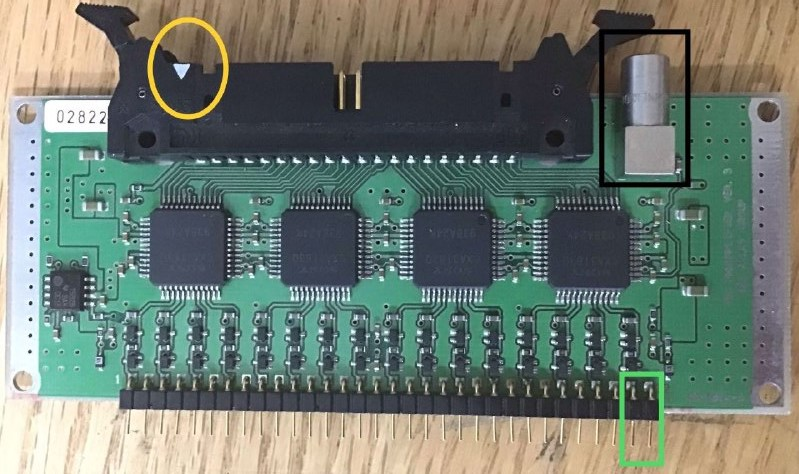
\includegraphics[scale=0.4]{asd.jpg}
	\caption{Placa ASD\cite{1999ATLASICs} (Amplificator Shaper Discriminator), encargada de captar los 16 pulsos provenientes de un detector y entregar pulsos digitales asociados a ellos en su salida. El detector se conecta en sus entradas DIP ubicadas en su extremo inferior, mientras que las señales LVDS de salida se ubican en el conector de 40 puertos para cable plano en su extremo superior.}
	\label{fig:asd}
\end{figure}

\begin{figure}[H]
	\centering
	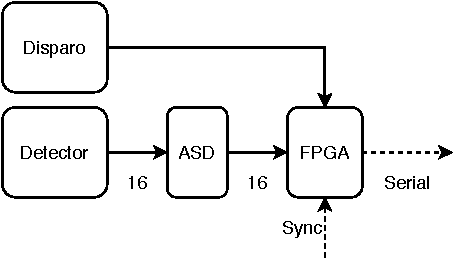
\includegraphics[scale=0.75]{fpga1.pdf}
	\caption{Diagrama de bloques utilizando una FPGA como alternativa de solución. Se indica una salida serial para transmitir los resultados del análisis básico a algún procesador o memoria de alguna etapa posterior. La señal de sincronización ``Sync'' tiene como objetivo sincronizar la recolección y procesamiento de eventos, para que estos sean consistentes entre detectores.}
	\label{fig:fpga1}
\end{figure}


La idea en esta alternativa de solución es guardar los pulsos provenientes de la placa ASD en memoria temporal hasta la llegada de una señal de disparo. Un módulo que maneja la memoria será el encargado de tomar los pulsos correspondientes al disparo recibido y liberar la memoria de aquellos datos ya leídos u obsoletos, entregando la información útil a una siguiente etapa. Los pulsos aceptados serán entonces relacionados como parte de un mismo eventos y se estimará la duración de estos, generando y guardando así un arreglo de datos con identificador de pulso y duración. La última etapa se encargará de efectuar una operación capaz de determinar la posición del evento a partir de las duraciones medidas y los pulsos detectados, comunicando así un arreglo básico y preprocesado que incluya posición espacial y magnitud aproximada.


\begin{figure}[H]
	\centering
	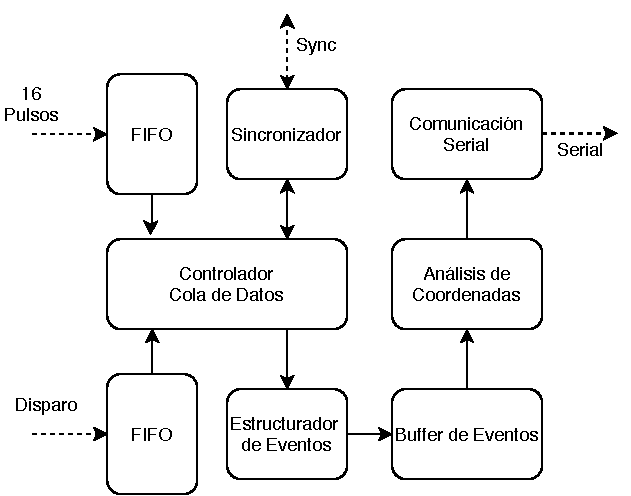
\includegraphics[scale=0.75]{fpga2.pdf}
	\caption{Representación de la lógica interna de la FPGA. Se incluye una cola de datos para las señales de disparo, para los pulsos digitales provenientes de la ASD y una memoria de almacenamiento temporal para los eventos ya estructurados. Los bloques controlador, estructurador y análisis cumplen las funciones de aceptar o descartar pulsos, cuantificar anchos de pulso a  los canales asociados y determinar coordenada del cruce de un muon respectivamente.}
	\label{fig:fpga2}
\end{figure}

Se espera que para lograr el escalamiento se incluya una señal para mantener la lectura de eventos sincronizada entre distintas FPGA. Además, se deberá incluir un modulo de comunicación para entregar la información captada a una etapa posterior con un análisis más detallado, encargado de reunir todos los eventos de diferentes FPGAs.

\section{Muestreo de Señales Digitales}
\label{sec:sampling}
Detalles de la etapa de muestreo de pulsos LVDS digitales provenientes de la interfaz de lectura. Diagramas del diseño de hardware, máquinas de estado, descripción del funcionamiento, entradas y salidas, recursos utilizados.

Primera etapa de diseño de hardware. Se reciben 16 canales digitales en formato LVDS, correspondientes a las señales de salida de la interfaz de lectura ASD. Estos pulsos se muestrean a una frecuencia de XHz y se almacenan en una memoria FIFO 

Para la implementación de este módulo, se 

\section{Discriminación de Eventos}
\label{sec:discriminator}
Diseño de etapa de discriminación, para distinguir pulsos reales de falsos positivos mediante señal de trigger externo. Diagramas, maquinas de estado y recursos asociados.

\section{Estructuración de Datos}
\label{sec:structure}
Diseño de la etapa de estructuración, para la organización de la información capturada en estructuras de datos coherentes. La información se asocia a canales y eventos. Diagramas, máquinas de estados, recursos.

\section{Análisis de Datos}
\label{sec:analysis}
Diseño de la etapa de análisis, para asociar cuadrantes y carga eléctrica a cada evento según los datos capturados. Diagramas, máquinas de estado, variables, recursos, descripción.


%\section{Sincronización}
%\label{sec:sync}


\section{Comunicación}
\label{sec:comm}
Diseño de etapa de comunicación serial, protocolo, caracteristicas, máquina de estado, diagramas, variables, recursos, descripciones.